\chapter{Asking Beverly Hills Billionaires How They Got So RICH!}

This chapter follows a School of Hard Knocks field lecture in Beverly Hills, but we should not read it as a mere parade of expensive objects and famous titles. The host begins with spectacle and surprise, then repeatedly asks us to look beneath the spectacle for operating structure: invention, margin, reinvestment, intermediation, leverage, diversification, balance-sheet strength, and finally organizational accountability. What emerges is not one single theory of wealth, but a small bank of mechanisms, introduced in sequence and motivated by the host's insistence on asking what actually produced the visible outcome.

\section{Spectacle, Method, and the Search for Mechanism}

The lecture opens with compressed future payoffs: a Rolls-Royce, a mafia confession, a Chipotle reveal. This is theater, but it is not empty theater. The point of the opening is to create enough narrative charge that the later explanations matter. Only after that does the host state the governing problem: we are in Beverly Hills, and the question is how fortunes were built.

That ordering matters. The lecture does not begin with a principle and then hunt for examples. It begins with outcomes and then asks us to reverse-engineer the machine. In that sense the opening behaves like a physical measurement: we are shown an effect and then asked for the mechanism that could have produced it.

There is a second structural point in the opening. The host does not promise one lesson. He promises a search across several wealth positions: inventor, intermediary, operator, professional, and scaled executive. The rest of the chapter should preserve that plurality.

\section{Invention, Margin, and Reinvestment}

The first fully developed case is the gel-nails founder. Here the lecture gives us the cleanest arithmetic of the entire episode. A product is invented; the product has extreme unit margin; borrowing is avoided; profit is recycled; distribution expands globally; personal consumption remains restrained even after success.

\begin{definition}
By \emph{unit economics} we mean the arithmetic at the level of one unit sold: price, direct cost, unit profit, and margin. The lecture's first serious mechanism of scale is built at precisely this level.
\end{definition}

The speaker gives the numerical core directly:
\begin{align}
P_{\mathrm{gel}} &= \$25, &
C_{\mathrm{gel}} &= \$1, \\
\pi_{\mathrm{gel}} &= P_{\mathrm{gel}}-C_{\mathrm{gel}}=\$24, &
m_{\mathrm{gel}} &= \frac{\pi_{\mathrm{gel}}}{P_{\mathrm{gel}}}=\frac{24}{25}\approx 0.96 .
\end{align}

This is the first place where the lecture becomes genuinely mathematical. A \(96\%\) gross margin does not by itself create a global company, but it changes the geometry of scale. When the speaker later says that he never had a line of credit, never had a mortgage, and never borrowed money in forty-four years, the claim is not mystical. It is made plausible by the unit economics.

Let us formalize the reinvestment logic in the minimal way:
\begin{equation}
K_{t+1}=K_t+\Pi_t-W_t ,
\end{equation}
where \(K_t\) is retained business capital after stage \(t\), \(\Pi_t\) is operating profit generated at that stage, and \(W_t\) is owner withdrawal.

The lecture begins this recursion with a very small initial condition:
\begin{equation}
K_0 \approx \$200 .
\end{equation}

If we suppress overhead for a moment and look only at the direct unit arithmetic, then the mechanism is almost embarrassingly simple:
\begin{align}
\Pi(n) &= 24n, \\
K_1 &= 200 + 24n - W_0 .
\end{align}
This is not a full business model; it is a stripped-down explanatory skeleton. But it captures why the lecture places so much emphasis on margin before it speaks about scale.

The same case then folds in a second principle: frugality after success. The Rolls-Royce is not denied, but it is discounted, literally and conceptually. We are told:
\begin{equation}
P_{\mathrm{car,list}} \approx \$520{,}000, \qquad
P_{\mathrm{car,auction}} \approx \$175{,}000, \qquad
\Delta P \approx \$345{,}000 .
\end{equation}
What matters is not the car as symbol, but the refusal to treat liquidity as a costume.

The distribution claim comes next:
\begin{equation}
N_{\mathrm{countries}} = 90 .
\end{equation}
This is the moment when the lecture widens from product to channel. The host asks whether product or distribution matters more, and the answer is not a reduction to one term. The business spreads because the product exists and because the founder travels, negotiates, and builds foreign markets.

\begin{figure}
\centering
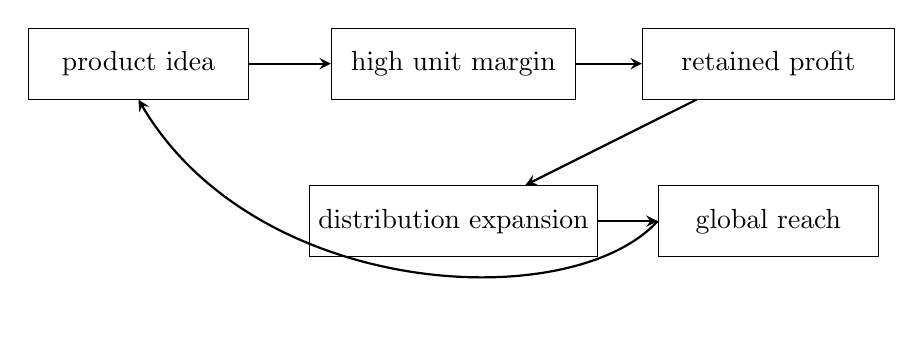
\begin{tikzpicture}[>=stealth]
\node[draw, rectangle, minimum width=2.8cm, minimum height=0.9cm] (a) at (0,0) {product idea};
\node[draw, rectangle, minimum width=3.1cm, minimum height=0.9cm] (b) at (4,0) {high unit margin};
\node[draw, rectangle, minimum width=3.2cm, minimum height=0.9cm] (c) at (8,0) {retained profit};
\node[draw, rectangle, minimum width=3.6cm, minimum height=0.9cm] (d) at (4,-2) {distribution expansion};
\node[draw, rectangle, minimum width=2.8cm, minimum height=0.9cm] (e) at (8,-2) {global reach};

\draw[->, thick] (a) -- (b);
\draw[->, thick] (b) -- (c);
\draw[->, thick] (c) -- (d);
\draw[->, thick] (d) -- (e);
\draw[->, thick] (e.west) .. controls (5.5,-3.2) and (1.5,-3.0) .. (a.south);
\end{tikzpicture}
\caption{Transcript-derived reconstruction of the first wealth mechanism: invention produces margin, margin produces retained profit, retained profit funds distribution, and distribution closes the loop by enlarging the reachable market.}
\end{figure}

\subsection{Question \& Answer}

\paragraph{Question.} How do we scale to very large revenue without borrowing money?

\paragraph{Answer.} The lecture's answer is not a general theorem, but a concrete mechanism. We begin with very favorable unit economics, retain rather than extract profit, and iterate the update rule
\[
K_{t+1}=K_t+\Pi_t-W_t.
\]
If withdrawals are modest and margins remain high, internal capital accumulation can finance further distribution and further sales. The speaker's point is therefore not merely that debt is avoidable in principle, but that certain businesses are structured so that retained profit can do almost all of the compounding work.

\section{Intermediation and Transfer Capture}

After the inventor comes the intermediary. The oil-and-gas operator does not describe himself as the discoverer of oil, nor as the final large capital owner. He describes himself as the man who puts the deals together. That is a different position in the machine.

The lecture's own language suggests a minimal formal object:
\begin{equation}
\mathcal I
=
\text{owner}
\longleftrightarrow
\text{dealmaker}
\longleftrightarrow
\text{operator/buyer}.
\end{equation}
The point is not that every intermediary becomes wealthy. The point is that a transfer bottleneck can be monetized. If wealth or control must pass through a junction, the junction itself can acquire value.

This is why the host asks whether the middleman becomes wealthy when wealth is transferred from one person to another. The oil-and-gas speaker does not answer with a theory, but with a practical confirmation: he is the one assembling the deals, and persistence is the key behavioral rule. One does not take the first no.

\begin{figure}
\centering
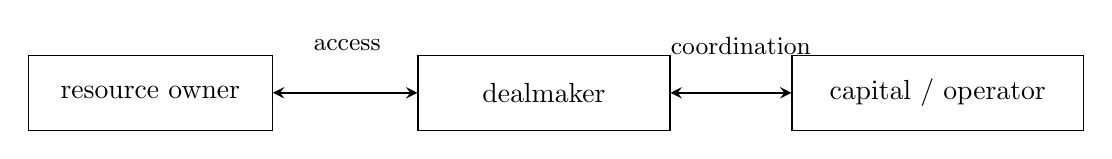
\begin{tikzpicture}[>=stealth]
\node[draw, rectangle, minimum width=3.1cm, minimum height=0.95cm] (o) at (0,0) {resource owner};
\node[draw, rectangle, minimum width=3.2cm, minimum height=0.95cm] (m) at (5,0) {dealmaker};
\node[draw, rectangle, minimum width=3.7cm, minimum height=0.95cm] (p) at (10,0) {capital / operator};

\draw[<->, thick] (o) -- (m);
\draw[<->, thick] (m) -- (p);

\node at (2.5,0.6) {\small access};
\node at (7.5,0.6) {\small coordination};
\end{tikzpicture}
\caption{Transcript-derived intermediation diagram. The lecture's claim is that value may be captured at the coordination node, not only at the endpoints.}
\end{figure}

The lecture keeps this mechanism grounded in biography. The speaker did not come from money; he was a high-school dropout; relationships mattered; and, in some lines of work, who one knows can dominate what one knows. The important thing for the notes is not to flatten this into vague networking advice. The structure is more specific: a market with complicated transfers can reward the agent who can repeatedly make the transfer happen.

\subsection{Question \& Answer}

\paragraph{Question.} Why does the middleman so often become wealthy?

\paragraph{Answer.} The lecture's answer is that the middle position may sit at a necessary point of coordination. If owner and operator cannot transact directly without search, trust, assembly, or negotiation, then the coordinating agent can earn a slice of the transfer. In symbols, the value lies not only in the endpoints but in the junction
\[
\text{owner}\longleftrightarrow \text{dealmaker}\longleftrightarrow \text{operator}.
\]
The host's insistence on sales and negotiation is therefore not ornamental. It is part of the mathematics of occupying the junction.

\section{Delegation, Leverage, and Accountability Under Pressure}

The lecture then escalates the middleman logic into a more extreme case through the former mafia operator. If we strip away the dramatic packaging, several mechanisms are introduced in rapid succession: revenue extraction at scale, negotiation from leverage, delegation, leadership, prison etiquette, and accountability.

The most numerical claim concerns gasoline:
\begin{equation}
q_{\mathrm{gas}}\approx 5\times 10^8\ \text{gallons/month}, \qquad
s_{\mathrm{gas}}\in[\$0.30,\$0.40]\ \text{per gallon}.
\end{equation}
This implies a very large monthly gross take:
\begin{equation}
\Pi_{\mathrm{gross,month}} = q_{\mathrm{gas}}\,s_{\mathrm{gas}}
\approx \$1.5\times 10^8 \text{ to } \$2.0\times 10^8.
\end{equation}
At the same time, the lecture reports weekly figures for the operation in the range
\begin{equation}
\Pi_{\mathrm{week}}\in[\$8\times 10^6,\$15\times 10^6].
\end{equation}

\begin{remark}
These numbers do not reconcile cleanly if read as a single accounting identity. The safest approach is to preserve them as speaker-reported quantities and not force a false consistency. The lecture uses them primarily to communicate scale, not to present a verified financial statement.
\end{remark}

If the gasoline arithmetic introduces scale, the delegation discussion introduces organizational form. The speaker's motto is almost axiomatic: do what you do best, delegate the rest. Here the lecture moves from money to structure. A leader is not merely a boss. A leader is followed willingly. This is not yet written as notation in the lecture, but later the Chipotle section will let us write it more sharply.

The negotiation-with-government story then inserts a second strong mechanism: leverage. The logic is very plain. The government wanted a conviction; the speaker had repeatedly beaten prior cases; therefore the bargaining problem was not symmetric. The lecture does not formalize that as game theory, but it unmistakably frames negotiation as a function of what the other side needs from you.

The prison section then seems at first like a digression, but it is really a lesson in local equilibrium. Respect is scarce, so small etiquette signals stabilize interaction. ``Please,'' ``thank you,'' and ``excuse me'' are not moral decorations in the story; they are low-cost devices for reducing escalation inside a high-friction social environment.

Finally, accountability appears in existential form rather than organizational form. The speaker says he was once accountable to an oath and a boss, and is now accountable to God and family. The underlying structure is already the one the lecture will later state more cleanly in management language: who or what one answers to changes the path of action.

\subsection{Question \& Answer}

\paragraph{Question.} What do delegation and leverage actually buy?

\paragraph{Answer.} Delegation enlarges the effective machine. One person ceases to be the sole executor and becomes the organizer of specialized work. Leverage changes the negotiation frontier: if the other side needs something that only we can provide, then the set of feasible outcomes changes in our favor. The lecture presents these two ideas through extreme biography, but the structural lesson is general.

\section{Access as a Product}

Midway through the lecture the host interrupts the interview rhythm and turns toward his own business. This interruption should be preserved, because it shows that access itself is being packaged as a product.

The numerical skeleton is straightforward:
\begin{equation}
F_{\mathrm{host}}\approx 12.7\times 10^6, \qquad
V_{\mathrm{month}}\approx 2\times 10^8, \qquad
N_{\mathrm{billionaires,US}}\approx 800, \qquad
N_{\mathrm{event}}=3.
\end{equation}
The offer is not simply ``watch wealthy people.'' The offer is scarcity and proximity: live calls, no recording, temporary window, direct access.

This section is not the doctrinal center of the lecture, but it is structurally important. The host is not only extracting lessons from wealth; he is also building a business from curation, access, attention, and urgency. In the chapter this should remain a short interlude, not a main theorem.

\section{From High Income to Industrial Ambition}

The Ghanaian plastic surgeon resets the tone. We move from intermediation and criminal leverage to professional excellence, personal values, and then to a larger industrial ambition. The lecture carefully stages this progression.

First we get the income anchor:
\begin{equation}
Y_{\mathrm{surgeon}}\approx \$9\times 10^6 \ \text{per year}.
\end{equation}
Second, the lecture places partner choice inside the economics of attention. The wrong marriage is described as a financial error because misalignment at home diverts energy from creation. The language is partly religious and partly practical, but the mechanism is not obscure: home instability taxes productive focus.

Third, the speaker refuses to stop at high income. He wants billionaire-scale wealth, and the path is diversification:
\begin{equation}
W_{\mathrm{total}} = W_{\mathrm{practice}} + W_{\mathrm{industrial}}.
\end{equation}
The second term is then named: a pharmaceutical plant in Ghana, intended to be the largest in sub-Saharan Africa. The lecture's point is not merely geographical ambition. It is a change of asset class. High-paid labor, even at extraordinary levels, is not yet the same thing as ownership of a large industrial machine.

\subsection{Question \& Answer}

\paragraph{Question.} Why is very high income still not the same thing as billionaire-scale wealth?

\paragraph{Answer.} Because the lecture distinguishes between income generated by skilled professional practice and wealth generated by ownership of scalable assets. In notation,
\[
W_{\mathrm{total}} = W_{\mathrm{practice}} + W_{\mathrm{industrial}}.
\]
The first term can be very large. But the lecture suggests that the second term is what changes the scale class of the problem.

\section{Chain Growth, Control, and the Fortress Balance Sheet}

The Chipotle CEO segment is the cleanest corporate block in the lecture. It begins with humble beginnings and reputation, then moves into scale arithmetic, non-franchised control, balance-sheet strength, and finally accountability.

The host first asks for the climb. We are told to read a career as a sequence of interviews, whether formal or not. Results produce credibility, and credibility in turn enlarges the range of future opportunities. This is narrative language, but it is already operational.

The numerical scale appears next:
\begin{align}
R_{\mathrm{Chipotle}} &\approx \$13\times 10^9 \ \text{per year}, \\
N_{\mathrm{Chipotle,now}} &\gtrsim 3800, \\
\Delta N_{\mathrm{year}} &\in [315,340], \\
N_{\mathrm{NA,target}} &\approx 7000 .
\end{align}
The most elementary growth rule is therefore
\begin{equation}
N_{t+1}=N_t+\Delta N_t.
\end{equation}

This lets us perform a rough horizon calculation. If the current base is just over \(3800\) restaurants and annual additions remain between \(315\) and \(340\), then the time to \(7000\) North American locations is on the order of a decade:
\begin{align}
\frac{7000-3800}{340} &\approx 9.4, \\
\frac{7000-3800}{315} &\approx 10.2.
\end{align}
This is a simple arithmetic check, not a forecast theorem. But it shows that the stated long-run target is of the same order as the stated annual expansion rate.

The next move is conceptual but still quantitative. Why no franchising? The answer is not an aesthetic dislike of franchises. It is a control decision made possible by the balance sheet:
\begin{equation}
C_{\mathrm{cash}}\gtrsim \$2\times 10^9, \qquad D_{\mathrm{debt}}=0.
\end{equation}
If internal capital is abundant and debt is absent, then the need to surrender operational control for growth capital becomes much smaller. The brand can remain internally governed.

The lecture then lands on its cleanest management statement: responsibility and accountability are not the same thing.

\begin{definition}
For a task \(T\), let \(\mathcal R(T)\) denote the set of parties who share responsibility for performing it, and let \(a(T)\) denote the unique accountable owner of the outcome, if such an owner exists.
\end{definition}

The lecture's principle becomes
\begin{equation}
|\mathcal R(T)|>1,\qquad a(T)=\varnothing
\quad \Longrightarrow \quad
\text{shared responsibility without accountability.}
\end{equation}
That is the cleanest portable abstraction in the whole episode. Many may work on a task; one must own the outcome.

\begin{figure}
\centering
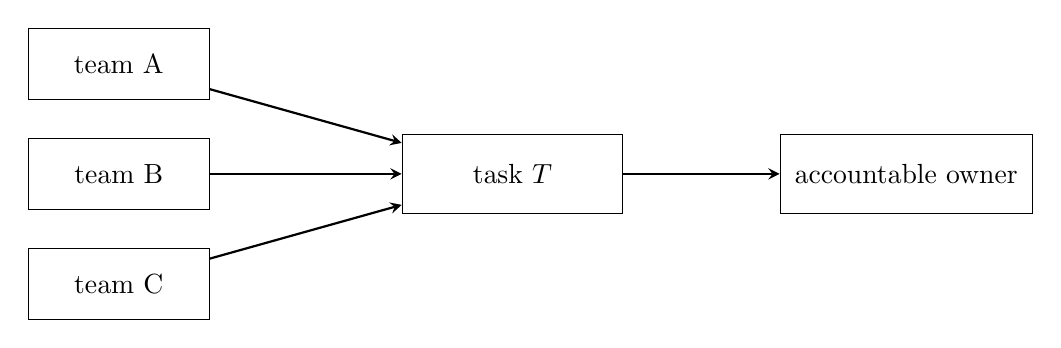
\begin{tikzpicture}[>=stealth]
\node[draw, rectangle, minimum width=2.3cm, minimum height=0.9cm] (r1) at (0,1.4) {team A};
\node[draw, rectangle, minimum width=2.3cm, minimum height=0.9cm] (r2) at (0,0) {team B};
\node[draw, rectangle, minimum width=2.3cm, minimum height=0.9cm] (r3) at (0,-1.4) {team C};

\node[draw, rectangle, minimum width=2.8cm, minimum height=1.0cm] (t) at (5,0) {task \(T\)};
\node[draw, rectangle, minimum width=3.2cm, minimum height=1.0cm] (a) at (10,0) {accountable owner};

\draw[->, thick] (r1) -- (t);
\draw[->, thick] (r2) -- (t);
\draw[->, thick] (r3) -- (t);
\draw[->, thick] (t) -- (a);
\end{tikzpicture}
\caption{Responsibility may be distributed, but accountability must terminate in one owner. This is the lecture's sharpest organizational distinction.}
\end{figure}

The final note in the Chipotle segment productively complicates the early frugality lesson. One cannot save one's way to prosperity, the speaker says. One must invest in the consumer experience and the team experience:
\begin{equation}
I_{\mathrm{consumer}} + I_{\mathrm{team}} \longrightarrow \text{outsized future returns}.
\end{equation}
This does not negate the earlier emphasis on waste avoidance. Rather, it distinguishes \emph{wasteful extraction} from \emph{strategic reinvestment}. The lecture ends, then, not with austerity alone, but with disciplined abundance.

\subsection{Question \& Answer}

\paragraph{Question.} Why refuse franchising when scale is already available?

\paragraph{Answer.} The lecture's answer is that franchising is one way to solve a capital and control problem, but it is not the only way. If internal capital is strong enough,
\[
C_{\mathrm{cash}}\gtrsim \$2\times 10^9, \qquad D_{\mathrm{debt}}=0,
\]
then expansion can be financed without giving up operational authority. The refusal to franchise is therefore part of a larger doctrine: growth should not come at the expense of brand integrity if the balance sheet already makes independent growth feasible.

\section{Summary}

The lecture begins with spectacle and ends with structure. In between, it gives us a small catalog of wealth mechanisms: invention with extreme margin, reinvestment without debt, intermediation at the transfer point, delegation under leverage, access sold as a product, professional income transformed by diversification, and chain growth financed by a fortress balance sheet.

What makes the episode worth writing down is not the celebrity of the interviewees, nor the glamour of Beverly Hills, but the way each case introduces a different answer to the same underlying question. How is visible wealth generated? The lecture's answer is that there is no single path, but there are recurring forms. We can write some of them down:
\[
K_{t+1}=K_t+\Pi_t-W_t, \qquad
\mathcal I=\text{owner}\longleftrightarrow \text{dealmaker}\longleftrightarrow \text{operator}, \qquad
|\mathcal R(T)|>1,\ a(T)=\varnothing.
\]
The details differ from case to case. The grammar, however, repeats.